%% Section II draft: Preliminaries.
%% Flow follows Park and Bang (IJCAS 22(11), 2024): the classical batch form of
%% the database-referenced problem first, then factor graph optimization as the
%% general machinery, so that Section III can put the two together.
%% Numbers: map amplitude along track from the line exports in
%% research/gtsam_poc/; interference magnitudes from the TL bootstrap logs.

\section{Problem Formulation}\label{sec:problem}
This section states what magnetic-anomaly navigation asks for in its classical
batch form, shows why the aircraft's own field prevents that form from being
answered directly, and states the problem solved in the rest of the paper.

\subsection{Batch map matching}\label{sec:batchmm}
Database-referenced navigation determines position by comparing a measured
profile against a stored map. Let $\mathbf{p}_{0:k}$ be the horizontal positions
of the aircraft over $k+1$ epochs, $z_{0:k}$ the scalar readings, and
$h(\cdot)$ the map lookup returning the field predicted at a position. The
classical batch estimate minimizes a profile-matching criterion, in mean
absolute or mean squared form,
\begin{equation}
J_{\mathrm{MAD}}=\frac{1}{k}\sum_{i=0}^{k}\big|\,z_i-h(\mathbf{p}_i)\big|,
\qquad
J_{\mathrm{MSD}}=\frac{1}{k}\sum_{i=0}^{k}\big(z_i-h(\mathbf{p}_i)\big)^{2},
\label{eq:mad}
\end{equation}
subject to the inertial navigation system supplying the increments between
consecutive positions,
\begin{equation}
\mathbf{p}_i-\mathbf{p}_{i-1}=\Delta\mathbf{p}^{\mathrm{ins}}_i,
\qquad i=1,\dots,k,
\label{eq:inshard}
\end{equation}
so that the search is over a rigid profile translated by the single unknown
initial state,
\begin{equation}
\hat{\mathbf{p}}_{0:k}=\arg\min_{\mathbf{p}_{0:k}} J .
\label{eq:batchmm}
\end{equation}
Terrain-referenced navigation is solved in this form
routinely~\cite{hollowell1990,cowie2008}, and the same form underlies the
magnetic case~\cite{canciani2016,canciani2017}.

We state~\eqref{eq:mad}--\eqref{eq:batchmm} as the reference formulation of
database-referenced navigation rather than as a competing method: airborne
magnetic-anomaly navigation is in practice run recursively, with a Kalman filter
or a particle filter aiding the inertial
solution~\cite{canciani2017,gnadt2022}, and those are the baselines compared
against in Section~\ref{sec:results}. The batch form is worth writing down
because it makes two things explicit that the recursive implementations leave
implicit, and both matter here. It shows what the map contributes, namely the
agreement between a measured profile and a stored one. And it treats the
inertial increment as the hard constraint~\eqref{eq:inshard}, which is the
assumption the factor graph of Section~\ref{sec:fgo} relaxes by admitting the
increment as one more piece of uncertain information.

What~\eqref{eq:mad} presumes is that the residual $z_i-h(\mathbf{p}_i)$ is small
and unstructured once the position is right. For a scalar magnetometer mounted
on an aircraft this is false, and by a wide margin. The measurement carries the
aircraft's own magnetic field, generated by permanent magnetization, by
currents induced in the airframe, and by eddy currents, all of which depend on
the aircraft attitude in the Earth field and therefore change continuously along
a line. On the five survey lines used in Section~\ref{sec:results} the map value
along the flown track varies with a standard deviation of
\SIrange{123}{327}{\nano\tesla} and a peak-to-peak swing of
\SIrange{586}{2377}{\nano\tesla}: that variation is the entire position signal.
Against it, the uncompensated field at a cabin-mounted magnetometer is
\SIrange{1729}{2081}{\nano\tesla} root-mean-square over the first
\SI{300}{\second} of flight. The interference is not a perturbation of the
signal, it is larger than the signal's full range.

Compensation is therefore not a refinement but a precondition. The classical
remedy is a calibration flight: a dedicated sequence of maneuvers at high
altitude, where the anomaly field is weak, from which the interference model is
fit once and then subtracted for the rest of the
mission~\cite{tolles1950,leliak1961,bickel1979}. That remedy is unavailable in
the situation this paper addresses. An aircraft that departs with an
uncalibrated installation, or whose interference has changed since its last
calibration, has no compensated measurement to feed
into~\eqref{eq:mad}. Estimating position then requires estimating the
compensation at the same time, from the same scalar stream that the map
matching consumes, and the two are coupled through that single stream: an error
in the compensation is indistinguishable, epoch by epoch, from an error in
position. We refer to this situation as a cold start, and it is the setting of
this paper.

\subsection{Problem statement}\label{sec:statement}
The situation just described fixes what has to be estimated and what may be
assumed. The aircraft carries a strapdown inertial navigation system whose
error grows without bound, a three-axis fluxgate, and a scalar magnetometer
whose reading is corrupted by the aircraft field. A gridded anomaly map of the
overflown region is available. No calibration flight has been made, so no
compensation model is known at takeoff, and no satellite navigation is
available at any point.

\begin{problem}[Joint navigation and compensation at a cold start]\label{prob:joint}
Given the scalar magnetometer measurements $z_{0:N}$, the fluxgate regressor
rows $\mathbf{A}_{0:N}$, the anomaly map $h$, the inertial mechanization, and a
prior $(\hat{\boldsymbol{\chi}}_0,\mathbf{P}_0)$ that assumes no prior
knowledge of the aircraft field, estimate the joint trajectory
$\boldsymbol{\chi}_{0:N}$ of inertial navigation errors $\mathbf{x}_k$ and
time-varying compensation coefficients $\boldsymbol{\beta}_k$, and do so with a
per-epoch cost that does not grow with flight duration, so that the estimate is
available on board.
\end{problem}

Three properties of Problem~\ref{prob:joint} shape the rest of the paper. It is
\emph{joint}, because the compensation cannot be measured separately from the
position it corrupts. It is \emph{underdetermined at any single epoch}, because
one scalar reading cannot separate a position error from a compensation error,
so the two are told apart only over a span of epochs. And it is
\emph{online}, because an estimator that must see the whole flight before
answering is of no use to the aircraft that flew it. The first two properties
call for an estimator that carries the compensation as a state and revises past
states as later data arrive; the third bounds how far into the past it may keep
revising. Sections~\ref{sec:fgo} and~\ref{sec:method} construct such an
estimator.

\section{Factor Graph Optimization}\label{sec:fgo}
Problem~\ref{prob:joint} is stated as maximum a posteriori (MAP) inference and
solved on a factor graph. This section sets out that machinery from the
beginning, since the structure of the graph is what allows the compensation to
be carried as a first-class unknown and the estimate to be produced in real
time.

\subsection{Variables, factors, and the graph}
An estimation problem consists of quantities that are unknown and pieces of
information that constrain them. In a factor graph the two are drawn as two
kinds of node~\cite{loeliger2004,dellaert2017}. A \emph{variable node} holds an
unknown, here the state $\boldsymbol{\chi}_k$ at one epoch. A \emph{factor node}
holds one piece of information, and an edge joins a factor to every variable
that piece of information involves. No edge joins two variables or two factors,
so the graph is bipartite, and a factor is a function only of the variables it
touches. Fig.~\ref{fig:fgbasic} shows the pattern for a short trajectory.

Three kinds of factor appear in any navigation graph, and they exhaust the ones
used in this paper. A \emph{prior} factor is unary and states what is believed
about a variable before any data: it fixes the otherwise free origin of the
estimate. A \emph{process} factor is binary and states how consecutive states are
related through the system dynamics and the inertial increments. A
\emph{measurement} factor is unary and states what a sensor reading predicts
about the state it was taken at. Writing $\mathbf{X}=\boldsymbol{\chi}_{0:N}$
for the collection of variables and $\mathbf{Z}$ for the data, the posterior
factors along exactly these edges,
\begin{equation}
p(\mathbf{X}\mid\mathbf{Z})\;\propto\;
p(\boldsymbol{\chi}_0)
\prod_{k=1}^{N}p(\boldsymbol{\chi}_k\mid\boldsymbol{\chi}_{k-1})
\prod_{k=0}^{N}p(z_k\mid\boldsymbol{\chi}_k),
\label{eq:posterior}
\end{equation}
which is written compactly as a product of factors
\begin{equation}
J(\mathbf{X};\mathbf{Z})=\prod_i\phi_i(\mathbf{X}_i;\mathbf{Z}),
\qquad
\hat{\mathbf{X}}=\arg\max_{\mathbf{X}}J(\mathbf{X};\mathbf{Z}),
\label{eq:prodfactors}
\end{equation}
with $\mathbf{X}_i$ the variables adjacent to factor $i$. The graph is a
picture of this factorization, and its sparsity is the problem's sparsity: each
factor constrains one or two states, never the whole trajectory at once.

\begin{figure}[t]
\centering
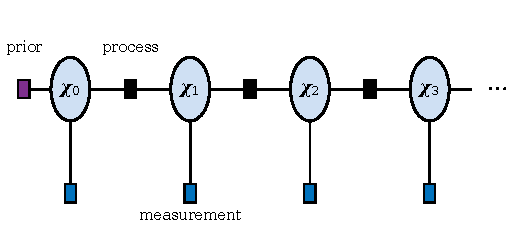
\includegraphics[width=\columnwidth]{figs/fig_fgbasic.pdf}
\caption{Factor graph of a short trajectory. Circles are variable nodes, one per
epoch; squares are factor nodes, each carrying one piece of information. The
unary prior anchors the first state, binary process factors link consecutive
states, and a unary measurement factor hangs from every state. A factor depends
only on the variables it is joined to, which is what makes the problem sparse.}
\label{fig:fgbasic}
\end{figure}

\subsection{From factors to least squares}
Each factor is modelled with a Gaussian kernel about its predicted value,
\begin{equation}
\phi_i(\mathbf{X}_i;\mathbf{Z})\propto
\exp\!\Big(-\tfrac{1}{2}\big\lVert g_i(\mathbf{X}_i)-\mathbf{z}_i\big\rVert^{2}_{\mathbf{P}_i}\Big),
\label{eq:kernel}
\end{equation}
where $g_i$ is the prediction associated with the datum $\mathbf{z}_i$,
$\mathbf{P}_i$ its covariance, and
$\lVert\mathbf{e}\rVert_{\mathbf{P}}=\sqrt{\mathbf{e}^{\top}\mathbf{P}^{-1}\mathbf{e}}$
the Mahalanobis norm. Taking the negative logarithm of~\eqref{eq:prodfactors}
turns the product into a sum and the maximization into a nonlinear least-squares
problem,
\begin{equation}
\hat{\mathbf{X}}=\arg\min_{\mathbf{X}}\sum_i
\big\lVert g_i(\mathbf{X}_i)-\mathbf{z}_i\big\rVert^{2}_{\mathbf{P}_i}.
\label{eq:nlls}
\end{equation}
The Mahalanobis weighting is what makes this sum meaningful. Inertial
increments, magnetic readings in nanotesla, and compensation coefficients have
different units and differ in magnitude by orders; they become comparable only
after each residual is divided by its own uncertainty. The covariance attached
to a factor is therefore not bookkeeping, it sets how much authority that piece
of information carries against every other; Section~\ref{sec:coldprior} sets the
one covariance a cold start is sensitive to.

\subsection{Solving the graph}
Because $g_i$ is nonlinear in the states, \eqref{eq:nlls} is solved
iteratively. Linearizing every residual about the current estimate
$\mathbf{X}^{(j)}$ and stacking gives
\begin{equation}
r(\mathbf{X})=
\begin{bmatrix} g_1(\mathbf{X}_1)-\mathbf{z}_1\\ \vdots\\
g_{N_f}(\mathbf{X}_{N_f})-\mathbf{z}_{N_f}\end{bmatrix},
\qquad
\mathcal{G}=\frac{\partial r}{\partial\mathbf{X}},
\label{eq:resstack}
\end{equation}
after which the Levenberg--Marquardt step
\begin{equation}
\Delta\mathbf{X}=-\big(\mathcal{G}^{\top}\mathcal{G}+\lambda\mathbf{I}\big)^{-1}
\mathcal{G}^{\top}r(\mathbf{X})
\label{eq:lm}
\end{equation}
is applied and the residuals are relinearized. The damping $\lambda$ interpolates
between Gauss--Newton and gradient descent and makes the iteration robust where
the problem is ill conditioned~\cite{dellaert2006}, which matters here because
the map term is strongly nonlinear.

Two consequences follow, and they are the reason for preferring this formulation
over a recursive filter. First, $\mathcal{G}$ inherits the sparsity of the graph:
a chain of process factors with unary measurements gives a block-bidiagonal
$\mathcal{G}$, so~\eqref{eq:lm} costs time linear in the number of states rather
than cubic. Second, every state is revised at every iteration. A filter commits
each state once, at the moment it is reached, and can never revisit it; the graph
relinearizes the whole set, so information that arrives late still corrects
estimates made early. In the cold start of Section~\ref{sec:batchmm} this is
exactly what is needed, because the compensation that explains the early
measurements is only identified after the aircraft has manoeuvred.

\subsection{Batch, fixed-lag, and incremental}
The formulation says nothing about how much of the flight $\mathbf{X}$ contains,
and that choice is the practical design variable. Taking $\mathbf{X}$ to be the
whole line gives the batch estimate: it uses every measurement and is the most
accurate, but it grows without bound and is available only after landing.
Restricting $\mathbf{X}$ to the states inside a bounded interval of the present,
and \emph{marginalizing} those that fall outside, gives a fixed-lag smoother
whose per-epoch cost does not grow with flight
duration~\cite{indelman2013,kaess2012}. Marginalization is not free: eliminating
a variable replaces its factors by a single dense factor on its former
neighbours, so what leaves the interval is summarized rather than discarded, and
it can no longer be revised.

Rebuilding and re-solving that interval from scratch at every epoch would waste
most of the work, since one new measurement changes little of a long chain.
Incremental solvers instead update the factorization in place, touching only the
part of it that the new data affect~\cite{kaess2012}. This is what makes a
fixed-lag smoother run at sensor rate, and it is the solver this paper uses;
Section~\ref{sec:incremental} states the construction and
Section~\ref{sec:lagdesign} measures what the length of the interval costs and
buys.
